\documentclass[12pt]{article}

\usepackage[T1]{fontenc}
\usepackage[polish]{babel}
\usepackage{listings}
\usepackage{graphicx}
\graphicspath{ {./images/} }
\usepackage{listings}
\usepackage[left=2.5cm, right=2.5cm, top=2.5cm]{geometry}
\usepackage{tocloft}
\renewcommand{\cftsecleader}{\cftdotfill{\cftdotsep}} % for sections

\title{Wycieki pamięci - analiza popularnych języków programowania}
\author{Mariusz Ziętek, Szymon Pituła}
\date{\today}

\begin{document}
\maketitle
\newpage
\tableofcontents
\newpage
\section{Wprowadzenie}
Wycieki pamięci to problem związany z alokacją i nie zwalnianiem pamięci programu, która nie jest już potrzebna.  Zjawisko to powoduje, że obszar pamięci który nie jest już używany przez program pozostaje oznaczony jako zajęty i nie może zostać ponownie wykorzystany. Problem ten jest najbardziej widoczny w aplikacjach, które działają ciągle lub przez długi okres czasu. Program taki będzie rezerwował coraz więcej pamięci, powodując znaczny spadek wydajności i w końcu zakończenie procesu. Wyciek pamięci jest stosunkowo trudny w wykryciu, ponieważ jego objawy nie są widoczne od razu po uruchomieniu programu. Problem ten jest spotykany w różnych językach programowania, w szeroko rozumianym programowaniu aplikacji. W swojej pracy chcielibyśmy przybliżyć ten problem czytelnikom, pokazać przyczyny i skutki wycieków pamięci oraz metody diagnozowania i unikania tego problemu w najpopularniejszych językach programowania: C/C++, Rust, Java, Python. Każdy z tych języków posiada inny system zarządzania pamięcią oraz wymaga innego udziału użytkownika w tym procesie.

\section{Metody i narzędzia do wykrywania wycieków}
Podstawowym narzędziem używanym przez nas do detekcji wycieków jest \textbf{Valgrind}. Jest to program dostarczający narzędzia do debugowania i profilowania działania programów. Najpopularniejszym narzędziem jest \textbf{Memcheck}, który będzie używany w tym projekcie najczęściej. Pozwala on na wykrycie błędów związanych z pamięcią (w tym wycieków), które mogą prowadzić do nieprzewidywalnego zachowania programu lub jego zakończenia. Istotną wadą programu jest jego wpływ na wydajność monitorowanej aplikacji. Valgrind potrafi spowolnić działanie programu nawet trzydziestokrotnie. W przypadku tego projektu nie jest to jednak duży problem, ponieważ przytoczone programy będą stosunkowo proste, aby przekaz był jak najbardziej przejrzysty.\\
Aby uruchomić aplikację z kontrolą Valgrind wystarczy dopisać odpowiednią flagę na przykład:
\begin{lstlisting}
valgrind --leak-check=yes myprog arg1 arg2
\end{lstlisting}
Powyższe polecenie pozwoli na uruchomienie narzędzia \textit{Memcheck} (domyślnie), wraz ze szczegółową kontrolą wycieków. Jeżeli Valgrind wykryje problem z pamięcią lub wyciek, zwróci odpowiednią wiadomość. Przykładowy raport wygląda następująco:
\begin{lstlisting}
  ==19182== Invalid write of size 4
  ==19182==    at 0x804838F: f (example.c:6)
  ==19182==    by 0x80483AB: main (example.c:11)
  ==19182==  Address 0x1BA45050 is 0 bytes after a block of size 
		40 alloc'd
  ==19182==    at 0x1B8FF5CD: malloc (vg_replace_malloc.c:130)
  ==19182==    by 0x8048385: f (example.c:5)
  ==19182==    by 0x80483AB: main (example.c:11)
\end{lstlisting}
\newpage
Informacje które tu widzimy to:
\begin{itemize}
  \item 19182 to ID procesu, zwykle nie jest ważne.
  \item Pierwsza linia ("Invalid write \ldots ") wskazuje na rodzaj problemu. W tym przypadku nieudana próba zapisu do pamięci.
  \item Poniżej znajduje się ślad stosu i nazwy funkcji mówiące o tym, gdzie wystąpił problem. Czytanie tej sekcji może być trudne w przypadku dużych programów, ułatwieniem może być czytanie od dołu.
\end{itemize}
Valgrind dzieli wycieki pamięci na kilka kategorii:
\begin{lstlisting}
==6051== LEAK SUMMARY:
==6051==    definitely lost: 16 bytes in 1 blocks
==6051==    indirectly lost: 0 bytes in 0 blocks
==6051==    possibly lost: 0 bytes in 0 blocks
==6051==    still reachable: 0 bytes in 0 blocks
==6051==    suppressed: 0 bytes in 0 blocks
\end{lstlisting}
\begin{itemize}
  \item definitely lost oznacza, że wyciek jest pewny i należy go naprawić.
  \item indirecty lost informuje o wycieku w strukturach bazujących na wskaźnikach. Przykład: jeżeli korzeń drzewa binarnego spowoduje \textit{definitely lost}, wszystkie dzieci spowodują \textit{indirectly lost}
  \item possibly lost zwykle oznacza to samo co \textit{definitely lost}, za wyjątkiem sytuacji, gdy jest on spowodowany umyślnie. Występuje gdy w programie znajdują się wskaźniki nie wskazujące na początek bloku.
  \item still reachable występuje w momencie, gdy program nie zwolnił pamięci, ale mógłby to zrobić. Zwykle nie jest to znaczący problem.
  \item suppressed wskazuje na błędy, które zostały wyciszone. Powinno się je ignorować.
\end{itemize}
Korzystając z programy Valgrind można zatem wyśledzić lokalizację błędu, określić jego przyczynę i rodzaj. Jest więc bardzo użytecznym narzędziem, które może pomóc w wyeliminowaniu błędów oprogramowania, a także w zwiększeniu wydajności. Dodatkowo Valgrind może działać na większości dostępnych platform i wspiera każdy język programowania. Narzędzie to powinno zatem być używane możliwie jak najczęściej (ograniczenia spowodowane są czasem działania programu), aby tworzone oprogramowania było jak najlepszej jakości. 
\newpage
\section{Wycieki pamięci w języku C/C++}
Konstrukcja tego języka pozwala na wykonanie wycieków pamięci na wiele sposobów. Wybraliśmy te z nich, które w możliwie czytelny sposób pokażą istotę problemu i takie, które są często popełniane. Poniżej przedstawione zostały wycieki związane z alokacją pamięci i zwalnianiem nieużywanego obszaru w przypadku korzystania ze wskaźników.
Do alokacji i zwalniania pamięci w języku C++ służą operatory \textit{new} oraz \textit{delete} (można także korzystać z operatorów jeżyka C, np. - \textit{alloc}, \textit{malloc}, \textit{free}. W języku tym odpowiedzialność za zarządzanie pamięcia leży po stronie programisty. Za pomocą \textit{new} rezerwuje się pamięć potrzebną do przechowania obiektu, a gdy ta nie jest już potrzebna należy ją zwolnić. Jeżeli programista nie użyje operatora \textit{delete} do zwolnienia pamięci, dojdzie do wycieku. Można to zaobserwować już w bardzo prostych programach. Poniższy przykład pokazuje różnicę w wykorzystaniu przez program pamięci w przypadku, gdy zostaje ona poprawnie zwolniona i w przypadku, gdy do zwolnienia nie dojdzie. Pierwszy fragment kodu obrazuje poprawne zarządzanie pamięcią:
\begin{lstlisting}
void problematic_function();
int main() {
    problematic_function();
    return 0;
}
void problematic_function(){
    int *data = new int;
    *data = 15;
    delete data;
}
\end{lstlisting}
Pamięć została zwolniona poprawnie, zatem nie powinien wystąpić wyciek. Potwierdzeniem tej tezy są wyniki programu Valgrind: \\\\
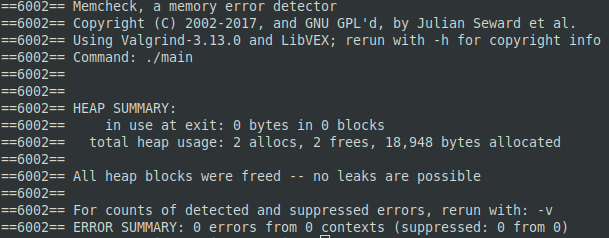
\includegraphics[scale=0.7]{cpp1nlVal} \\\\
Raport Valgrind mówi o tym, że zaalokowano i zwolniono dwie struktury, zatem wyciek nie jest możliwy. Całkowita użyta przez program pamięć to 18,948 bajtów. 
\newpage
\noindent
W kolejnym kroku z kodu programu zostanie usunięta linia odpowiedzialna za zwolnienie pamięci:
\begin{lstlisting}
void problematic_function();
int main() {
    problematic_function();
    return 0;
}
void problematic_function(){
    int *data = new int;
    *data = 15;
}
\end{lstlisting}
Zmieniony program zostaje przetestowany przez Valgrind i wyniki są następujące: \\\\
\includegraphics[scale=0.5]{cpp1lVal} \\\\
Tym razem Valgrind informuje o wycieku. Według raportu po zakończeniu programy w użyciu zostały 4 bajty, co zgadza się z rozmiarem niezwolnionej liczby całkowitej. Dodatkowo mamy też informację, że wyciek jest definitywny, czyli bezwzględnie wystąpił. Valgrind informuje także o miejscu wystąpienia błędu. Korzystając z tej informacji można szybko zlokalizować błąd. Z informacji wynika, że przyczyną jest operator \textit{new} w funkcji \textit{problematicfunction()} wywołanej w \textit{main()}. Informacja ta jest oczywiście prawdziwa, co łatwo zauważyć analizując kod programu.
\newpage
\noindent
Kolejny przykład prezentuje często popełniany błąd, który łatwo popełnić. 
\begin{lstlisting}
struct problematicStructure{
    int indexNumber;
    float *grades = new float[1000];
};

int main() {

    problematicStructure *s1 = new problematicStructure();
    delete s1;
    return 0;
}
\end{lstlisting}
Mogłoby się wydawać, że program jest wykonany poprawnie. Struktura została zaalokowana i zwolniona. Valgrind jednak pokaże, że istnieje wyciek pamięci.\\\\
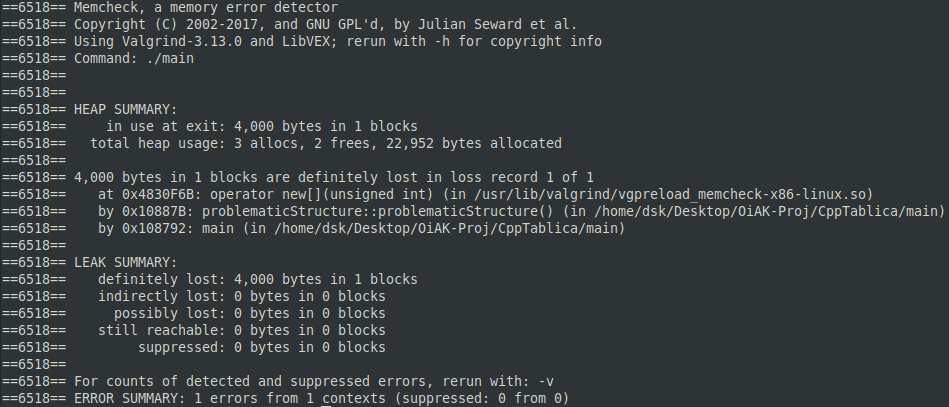
\includegraphics[scale=0.5]{cpp2lVal} \\\\
Istotą problemu jest to, że należy usunąć \textbf{całą} zarezerwowaną pamięć. Zdarza się, że programista usunie strukturę bądź klasę której już nie potrzebuje, ale zapomni o jej wewnętrznych zasobach. Valgrind informuje o definitywnym wycieku 4000 bajtów, co odpowiada 1000 liczb typu float. W przypadku usunięcia tablicy, ale nie zwolnienia pamięci zajmowanej przez strukturę, Valgrind Również znajdzie wyciek. W tym przypadku będzie to jednak tylko 8 bajtów, odpowiadających rozmiarowi struktury.
\newpage
\noindent
Aby całkowicie wyeliminować wyciek pamięci w programie należy zwolnić zarówno strukturę jak i tablicę w niej zawartą, pamiętając o odpowiedniej kolejności: 
\begin{lstlisting}
struct problematicStructure{
    int indexNumber;
    float *grades = new float[1000];
};

int main() {

    problematicStructure *s1 = new problematicStructure();
    delete[] s1->grades;
    delete s1;
    return 0;
}
\end{lstlisting}
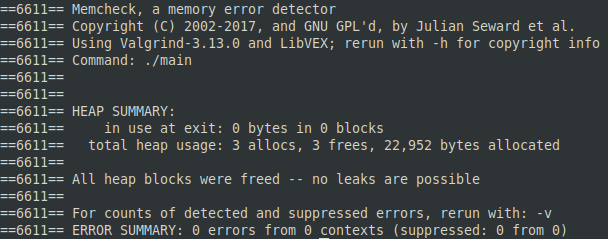
\includegraphics[scale=0.7]{cpp2nlVal} \\\\
Powyższe przykłady obrazują, że w języku C oraz C++ do wycieku pamięci można doprowadzić w bardzo prosty sposób. Odpowiedzialność za zarządzanie pamięcią spoczywa na programiście, zatem unikanie wycieków może być trudne. Dodatkowo pokazane przykłady obejmują wąski zakres problemu, który występuje w tym języku. Szczególnie więc warto korzystać z narzędzi takich jak Valgrind, Address Sanitizer, czy menadżer zasobów Visual Studio.
\newpage
\noindent
\section{Wycieki pamięci w języku Rust}
Rust różni się od innych języków programowania sposobem zarządzania pamięcią. Sprawdzanie poprawności kodu pod kątem błędnego użycia pamięci odbywa się już na etapie kompilacji, a nie po uruchomieniu aplikacji. Rust nie posiada Garbage Collectora, ale wprowadza mechanizm zwany \textbf{Ownership}. Własność ta tak jak w przypadku C++ zmusza programistę do ręcznego zarządzania pamięcią, jednak istotną różnicą jest to, że program napisany w Rust nie skompiluje się, jeżeli wykryty zostanie błąd. Dodatkowo Ownership ułatwia zarządzanie pamięcią, pozwalając na tylko jednego właściciela obiektu, a także poprzez automatyczne zwalnianie zasobów. Oznacza to, że deklarując zmienną, przypisywany jest do niej Ownership, czyli zmienna staje się właścicielem pewnego fragmentu pamięci. Pamięć ta zostanie automatycznie zwolniona w momencie wyjścia poza zakres użycia zmiennej (np. po wyjściu z funkcji). Rust wydaje się zatem być językiem znacznie bardziej bezpiecznym niż C++. Czy to oznacza, że wyciek pamięci jest niemożliwy? Tylko w teorii. Dokumentacja Rust mówi o tym, że język stara się kontrolować wycieki, ale nie jest to całkowicie możliwe, poprzez nieprzewidywalną naturę tego zjawiska. \\\\
W języku Rust najłatwiej zobrazować wyciek pamięci wywołując go specjalną funkcją \textit{mem::forget}. Powoduje ona, że Rust usunie zmienną, ale nie uruchomi jej destruktora.
\end{document}